\subsubsubsubsection{Road sign}
\begin{figure}[h]
\centering
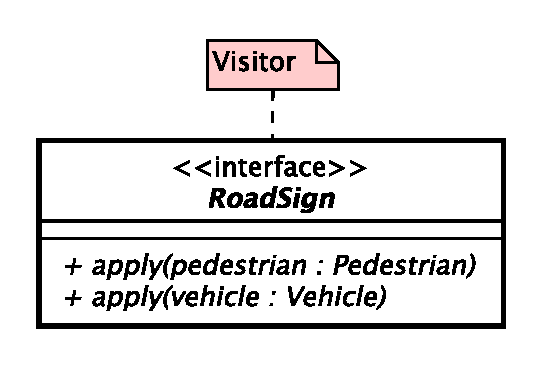
\includegraphics[scale=0.6,keepaspectratio]{images/solution/app/backend/road_sign.eps}
\caption{\pPassive::RoadSign}
\label{fig:sd-app-road-sign}
\end{figure}
\FloatBarrier
\begin{itemize}
  \item \textbf{\descr} \\
    It represents an interface which expose a method to apply the behaviour of a specific road sign.
  \item \textbf{\ops}
  \begin{itemize} 
    \item[+] \texttt{\textit{apply(pedestrian: Pedestrian)}} \\
Abstract method which will implement the effect of a road sign on a Pedestrian.
    \item[+] \texttt{\textit{apply(vehicle: Vehicle)}} \\
Abstract method which will implement the effect of a road sign on a Vehicle.
  \end{itemize}
\end{itemize}
